% !TeX root = ../main.tex

\chapter{Methodology}\label{chapter:methodology}
Our goal here is to build a system that is capable of accurately predicting when the user is going to eat.
This can be achieved by building predictive models and training them on user data.
But, in order to this, we first need to collect data on user's eating patterns.
This process is called dietary assesment.
There are many methods for dietary assesment.
Here, we will be focusing on a mobile-based solution:
We will build a dialog agent that allows for instant logging of a user's dietary intake.
Afterwards, using the gathered data, we will build a machine learning pipeline that predicts the time of the next entry.

\section{Dialog Agent}
\subsection{Design}
\subsubsection{Chatbot Architecture}
We will be building a task-oriented dialog agent.
The task is to understand the eating patterns of the user and make future predictions.
Let's take a look at our task from a frame-based perspective.
What information do we need from the user in order to accomplish this task?
There are many answers to this question with varying complexity.
Keeping the scope of the thesis in mind, we contruct a simple frame shown in \autoref{tab:main_frame}

\begin{table}[htbp]
  \caption[Frame for Logging Dietary Intake]{Frame for Logging Dietary Intake}\label{tab:main_frame}
  \centering
  \begin{tabular}{l|l|l}
    Slot&Type&Explanation\\ \toprule
    User Id&int&A user's identifying integer \\ \hline
    Meal Time&Time&Time of the meal\\ \hline
    Meal Date&Date&Date of the meal\\ \hline
    Meal Type&int&Type of the meal, 0 for Snack and 1 for Full Meal \\ \hline
  \end{tabular}
\end{table}

Now we need to come up with a question for every slot in the frame.
\autoref{tab:logging_questions} shows these questions.
We don't assign questions to User Id and Meal Date slots, as they are meant to be infered from the context.

\begin{table}[htbp]
  \caption[Question for Logging Dietary Intake]{Questions for Logging Dietary Intake}\label{tab:logging_questions}
  \centering
  \begin{tabular}{l|l|l}
    Slot&Questions\\ \toprule
    User Id&-\\ \hline
    Meal Time&When was this meal/snack?\\ \hline
    Meal Date&-\\ \hline
    Meal Type&Was this a meal or a snack?\\ \hline
  \end{tabular}
\end{table}

Based on these questions, we build a simple control structure shown in \autoref{fig:logging_control}.
This control structure follows a mixed initiative approach, 
allowing the user to deliver the information in any sequence.

\usetikzlibrary{automata,positioning}
\tikzstyle{state} = [rectangle,
                    text width=5cm,
                    align = center,
                    draw=black!80,
                    fill=black!5,
                    very thick]
\tikzstyle{control} = [node distance=2cm,
                      trim left=(0),
                      trim right=(0),
                      >=stealth,
                      shorten >=1pt,
                      auto]
\begin{figure}[htbp]
  \centering
  \caption[Control Structure for Meal Logging]{Control Structure for Meal Logging}\label{fig:logging_control}
  \scalebox{0.6}{
  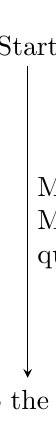
\begin{tikzpicture}[control]
    \node (0) {Start};
    \node (1) [below left =of 0, xshift=-1cm] [state] {Was this a meal or a snack?};
    \node (2) [below right =of 0, xshift=1cm] [state] {When was this \{1:meal, 0:snack\}[<meal\_type>]?};
    \node (3) [below =of 0, yshift= -2cm] {Save into the database};
    \path[->]
      (0) edge node [swap, midway] {Meal Time acquired} (1)
      (0) edge node [midway] {Meal Type acquired} (2)
      (0) edge node [midway, text width=3cm] {Meal Time and Meal Type acquired} (3)
      (1) edge node [swap, midway] {Meal Type acquired} (3)
      (2) edge node [midway] {Meal Time acquired} (3);
  \end{tikzpicture}}
\end{figure}


But what if a user makes a faulty entry and wants to remove it?
We need to include a system that let's users remove entries.
Knowing the date and time of an entry is enough to remove it, so we construct the frame shown in \autoref{tab:remove_frame}.

\begin{table}[htbp]
  \caption[Frame and Questions for Removing Entries]{Frame and Questions for Removing Entries}\label{tab:remove_frame}
  \centering
  \begin{tabular}{l|l|l}
    Slot&Type&Questions\\ \toprule
    User Id&int&-\\ \hline
    Meal Date&Date&What was the date of this entry?\\ \hline
    Meal Time&Time&What was the time of this entry?\\ \hline
  \end{tabular}
\end{table}

Based on \autoref{tab:remove_frame}, we construct a control structure for entry removal, shown in \autoref{fig:remove_control}.

\begin{figure}[htbp]
  \centering
  \caption[Control Structure for Removing Entries]{Control Structure for Removing Entries}
  \label{fig:remove_control}
  \scalebox{0.5}{
  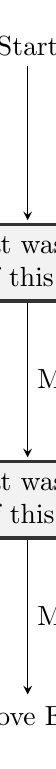
\begin{tikzpicture}[control]
    \node (0) {Start};
    \node (1) [below =of 0] [state] {What was the date of this entry?};
    \node (2) [below =of 1] [state] {What was the time of this entry?};
    \node (3) [below =of 2] {Remove Entry};
    \path[->]
      (0) edge (1)
      (1) edge node [midway] {Meal Date acquired} (2)
      (2) edge node [midway] {Meal Time acquired} (3);
  \end{tikzpicture}}
\end{figure}

\newpage

Before logging any meals, however, we need to know some things about the user.
For example, user's timezone.
It is not possible to obtain accurate time information without knowing the user's time zone.
For the overall system, we also need to know the user's dietary goal.
Both of these informations must be acquired at first contact with the user.
Based on this, we build the frame and questions seen in \autoref{tab:reg_frame} for user registration.
We derive the timezone from user's location.
The dietary goal is represented as an integer, corresponding to:

0: Lose Weight

1: Mainting Weight

2: Gain Weight


\begin{table}[htbp]
  \caption[Frame and Questions for User Registration]{Frame for User Registration}
  \label{tab:reg_frame}
  \centering
  \begin{tabular}{l|l|l}
    Slot&Type&Question\\ \toprule
    User Id&int&-\\ \hline
    Timezone&text&Please share your location with me so I can find your timezone.\\ \hline
    Goal&int&Please select your goal.\\ \hline
  \end{tabular}
\end{table}

Based on \autoref{tab:reg_frame}, we construct the control structure shown in \autoref{fig:reg_control}

\begin{figure}[htbp]
  \centering
  \caption[Control Structure for User Registration]{Control Structure for User Registration}
  \label{fig:reg_control}
  \scalebox{0.5}{
  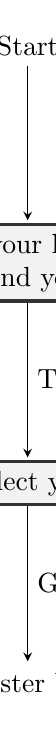
\begin{tikzpicture}[control]
    \node (0) {Start};
    \node (1) [below =of 0] [state] {Plese share your location with me so I can find your timezone.};
    \node (2) [below =of 1] [state] {Please select your goal.};
    \node (3) [below =of 2] {Register User};
    \path[->]
      (0) edge (1)
      (1) edge node [midway] {Timezone acquired} (2)
      (2) edge node [midway] {Goal acquired} (3);
  \end{tikzpicture}}
\end{figure}


We also contruct two more control structres, for changing timezone and goal settings, shown in \autoref{fig:change_control}

\begin{figure}[htbp]
  \centering
  \caption[Control Structures for Changing Timezone and Goal]{Control Structures for Changing Timezone and Goal}
  \label{fig:change_control}
  \scalebox{0.5}{
  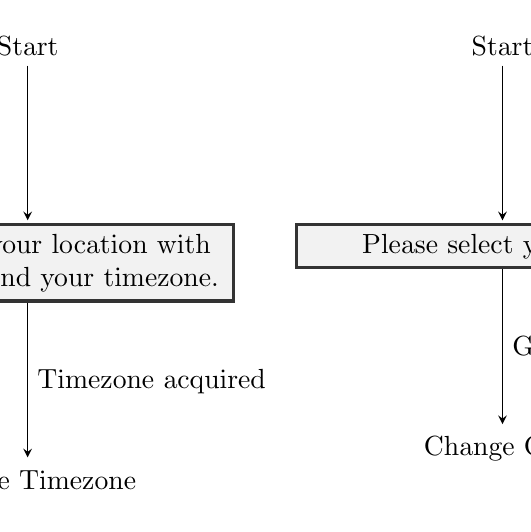
\begin{tikzpicture}[node distance=2cm,
                      trim left=(0),
                      trim right=(3),
                      >=stealth,
                      shorten >=1pt,
                      auto]
    \node (0) {Start};
    \node (1) [below =of 0] [state, text width=5cm] {Plese share your location with me so I can find your timezone.};
    \node (2) [below =of 1] {Change Timezone};
    \node (3) [right =of 0, xshift=3cm] {Start};
    \node (4) [below =of 3] [state] {Please select your goal.};
    \node (5) [below =of 4] {Change Goal};
    \path[->]
      (0) edge (1)
      (3) edge (4)
      (1) edge node [midway] {Timezone acquired} (2)
      (4) edge node [midway] {Goal acquired} (5);
  \end{tikzpicture}}
\end{figure}

We also need to send messages at predicted times and ask for feedback on the prediction.
The control structure for sending messages and asking for feedback is shown in \autoref{fig:send_control}.

\begin{figure}[htbp]
  \centering
  \caption[Control Structure for Sending Messages and Asking for Feedback]{Control Structure for Sending Messages and Asking for Feedback}
  \label{fig:send_control}
  \scalebox{0.5}{
  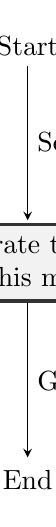
\begin{tikzpicture}[control]
    \node (0) {Start};
    \node (1) [below =of 0] [state] {Please rate the timing of this message.};
    \node (2) [below =of 1] {End};
    \path[->]
      (0) edge node [midway] {Send Message} (1)
      (1) edge node [midway] {Get Feedback} (2);
  \end{tikzpicture}}
\end{figure}

Bringing all these control structures together, we end up with a final structure describing the entire system, shown in \autoref{fig:system_control}
\begin{figure}[htbp]
  \centering
  \caption[Control Structure for the Entire System]{Control Structure for the Entire System}
  \label{fig:system_control}
  \scalebox{0.6}{
  
\begin{tikzpicture}[control]
    \node (0) {Start};
    \node (1) [below =of 0] [state] {Plese share your location with me so I can find your timezone.};
    \node (2) [below =of 1] [state] {Please select your goal.};
    \node (3) [below =of 2] {Register User};
    \node (4) [below =of 3] [state] {Idle};
    \node (5) [below =of 4] {Log a new entry};
    \node (6) [above right =of 4] {Remove an entry};
    \node (7) [above left =of 4] {Change Timezone};
    \node (8) [below left =of 4] {Change Goal};
    \node (9) [below left =of 5, xshift=-1cm] [state] {Was this a meal or a snack?};
    \node (10) [below right =of 5, xshift=1cm] [state] {When was this \{1:meal, 0:snack\}[<meal\_type>]?};
    \node (11) [below =of 5, yshift= -2cm] {Save into the database};
    \node (12) [right =of 6] [state] {What was the date of this entry?};
    \node (13) [above=of 12] [state] {What was the time of this entry?};
    \node (14) [above =of 13] {Remove Entry};
    \node (15) [above left =of 7] [state, text width=5cm] {Plese share your location with me so I can find your timezone.};
    \node (16) [above =of 15] {Change Timezone};
    \node (17) [left =of 8] [state, text width=5cm] {Plese select your goal.};
    \node (18) [above =of 17] {Change Goal};
    \node (19) [right =of 4, xshift=2cm] [state] {Please rate the timining of this message.};
    \path[->]
      (0) edge (1)
      (1) edge node [swap, midway] {Timezone acquired} (2)
      (2) edge node [swap, midway] {Goal acquired} (3)
      (3) edge (4)
      (4) edge (5)
      (4.north east) edge (6)
      (4) edge (7)
      (4) edge (8)
      (5) edge node [swap, midway] {Meal Time acquired} (9)
      (5) edge node [midway] {Meal Type acquired} (10)
      (5) edge node [midway, text width=3cm] {Meal Time and Meal Type acquired} (11)
      (9) edge node [swap, midway] {Meal Type acquired} (11)
      (10) edge node [midway] {Meal Time acquired} (11)
      (11.south) edge [bend right=90, looseness=5](4.south east)
      (6) edge (12)
      (12) edge node [swap, midway] {Meal Date acquired} (13)
      (13) edge node [swap, midway] {Meal Time acquired} (14)
      (14.west) edge (4.north)
      (7) edge (15)
      (15) edge node [midway] {Timezone acquired} (16)
      (8) edge (17)
      (17) edge node [midway] {Goal acquired} (18)
      (16.east) edge (4.north)
      (18.east) edge (4.west)
      (4.north east) edge [bend left=15] node [pos =0.7] {Send message} (19.north west)
      (19.south west) edge [bend left=15] node [swap, pos=0.1] {Get Feedback} (4.south east);

  \end{tikzpicture}}
\end{figure}

\subsubsection{Information Extraction}
We need to extract relevant information from the user's messages in order to fill the slots.
This mainly concerns extracting time and type of an entry.
For other information, we will be taking advantage of Telegram Chatbot API's various functionalities, which will be explained in the next subsection.
We will be performing information extraction primarily with the help of regular expressions.
All the mentioned regular expressions need the X flag set, allowing for whitespace within the expression.
For extracting the type of the entry (i.e. meal or snack) we will be using the regular expression shown in \autoref{fig:re_type}.

\begin{figure}[htpb]
  \centering
  \begin{tabular}{c}
  \begin{lstlisting}[language=python]
type_pattern = r'''\b
(?:
(?P<meal>meal|breakfast|lunch|dinner)|
(?P<snack>snack|small|little|few)
)
\b'''
  \end{lstlisting}
  \end{tabular}
  \caption[Regular Expression for Extracting Entry Type]{Regular Expression for Extracting Entry Type}
  \label{fig:re_type}
\end{figure}

This regular expression matches a word from a set of words between word boundries.
If the matched word is meal, breakfast, lunch or dinner; the extracted type is set to meal.
If the matched word is snack, small, little or few; the extracted type is set to snack.


\begin{figure}[htpb]
  \centering
  \begin{tabular}{c}
  \begin{lstlisting}[language=python]
r'''\b
(?:at\s*)?
(?:
(?P<hours>
[01]?\d|2[0-3])
(?:[:\.\s]
(?P<minutes>
[0-5]?\d))?
(?P<AmPm>\s*[ap]m)?
|(?P<hours_alt>[01]\d|2[0-3])(?P<minutes_alt>[0-5]\d))
\b'''
  \end{lstlisting}
  \end{tabular}
  \caption[Regular Expression for Extracting Absolute Temporal Expressions]{Regular Expression for Extracting Absolute Temporal Expressions}
  \label{fig:re_time_a}
\end{figure}

\begin{figure}[htpb]
  \centering
  \begin{tabular}{c}
  \begin{lstlisting}[language=python]
r'''\b
(?P<hours>
(?:half(?:\s*\b(?:a|an|)\b\s*)?|
\ba\b|\ban\b|
1?[0-9]|2[0-4])?
\s*
(?:h|hour)s?)?
\s*
(?P<minutes>
(?:\ba\b|\ban\b|
[0-9]{1,2})
\s*
(?:m|min|minute)s?\b)?
\s*
(?:ago|before|prior)
\b'''
  \end{lstlisting}
  \end{tabular}
  \caption[Regular Expression for Extracting Relative Temporal Expressions]{Regular Expression for Extracting Relative Temporal Expressions}
  \label{fig:re_time_r}
\end{figure}

For extracting the time of the entry, we use two different regular expressions: 
one for absolute temporal expressions shown in \autoref{fig:re_time_a}, and another for relative temporal expressions shown in \autoref{fig:re_time_r}.
From here on, in order to avoid confusion between regular expressions and temporal expressions, 
we will be referring to the regular expressions as extractors.

Absolute time extractor matches any phrase that has a hour part; a single or double digit number between 0 and 23.
It also optionally matches a minutes part; a single or double digit number between 0 and 59.
The hours and minutes parts need to be seperated by a delimiter; either a colon, a period or a space.
After the hours and minutes parts, if there is a phrase signifying 12 hour format (am-pm), the phrase is also matched.
Alternatively, the extractor also matches military time; a four digit representation where the first two digits signigy hours and last two digits signify minutes. (e.g 2000)

Relative time extractor matches phrases followed by a trigger word.
This word can be ago, before or prior.
Preceeding the trigger word, hours part, minutes part or both can be matched.
Hours part is a single or double digit number between 0 and 24, followed by a word signifying hours (h, hours etc.).
Minutes part is a single or double digit number between 0 and 99, followed by a word singifying minutes (min, minutes etc.).
Additionally, the extractor also matches the word 'half' if it preceeds the hours part.
After the extraction, relative time is normalized based on the user's timezone.

When we get a message from the user, we first run the relative time extractor on the text.
To understand why, consider the phrase `I ate 5 minutes ago'.
While this is clearly a relative temporal expression, it is also matched by absolute temporal expression.
However, relative time extractor involves trigger words.
This means that if the relative time extractor matches a phrase, it is safe to assume that the phrase is a relative temporal expression.

We have a final regular expression shown in \autoref{fig:re_log}
We use this expresssion to determine if a user is trying to log an entry.

\begin{figure}[htpb]
  \centering
  \begin{tabular}{c}
  \begin{lstlisting}[language=python]
r'''\b
(eat|ate|eaten|food)
\b'''
  \end{lstlisting}
  \end{tabular}
  \caption[Regular Expression for User Intent]{Regular Expression for User Intent}
  \label{fig:re_log}
\end{figure}

Similar to the type expression, this expression matches a word from a set of words between word boundries.
The words that can be matched are; eat, ate, eaten and food.
We use this expression only if both time and type expressions fail to match anything.
This is because if the previous expressions match a phrase, then the intent is already established.

\subsection{Implementation}
Instead of developing a stand-alone application, we build our dialog agent as a Telegram chatbot.
This makes the development process significantly easier.
Instead of focusing on application design, we can fully focus on our dialog agent.
We build our dialog agent using Python 3 and python-telegram-bot library, which provides a python interface for Telegram Bot API.

In the previous subsection, we have mentioned that we would be using some Telegram Bot API functionalities in order to make information extraction easier. 
We will start this subsection by explaining these functionalites.
Next we will move on to the control structure of a Telegram chatbot.
Finally, we will briefly mention some other libraries that are also used in our implementation.
\subsubsection{python-telegram-bot Library}
\subsubsection{Telegram Bot API}
There are some Telegram Bot functionalities that we make use of in order to make information extraction easier.
First of those are the chatbot commands.
Telegram Bot API allows user to perform actions via commands.
A command is a string of alphanumerical characters and underscores, all of which is preceeded by a '/' character.
For example, '/help', '/set\_nickname' or '/command3' or all viable commands.
In our system, we use commands to start any operation other than logging an entry.
We implement a total of four commands:

\paragraph{/start} command is automatically called when a user messages our chatbot for the first time. This command initiates the registration sequence shown in \autoref{fig:reg_control}. Registered user's can not call this command.

\paragraph{/change\_timezone} command initiates the timezone changing sequence shown in \autoref{fig:change_control}. 
This command can be called at anytime after the registration. 

\paragraph{/change\_goal} command initiates the goal changing sequence also shown in \autoref{fig:change_control}. 
This command can also be called at anytime after the registration.

\paragraph{/remove\_entry} command initiates the entry removal sequence shown in \autoref{fig:remove_control}. 
This command can also be called at anytime after the registration.

\begin{figure}[htbp]
\begin{minipage}{.5\textwidth}
	\centering
        \captionsetup{width=\linewidth}
	\includegraphics[scale=0.2]{figures/commands}
        \caption{Screenshot Showing Available Commands for the Chatbot}
	\label{fig:commands}
\end{minipage}%
\begin{minipage}{.5\textwidth}
	\centering
        \captionsetup{width=.9\linewidth}
	\includegraphics[scale=0.2]{figures/keyboard}
        \caption{Screenshot Showing an Inline Keyboard}
	\label{fig:keyboard}
\end{minipage}
\end{figure}

We also make use of Inline-Keyboard functionality to decrease information extraction effort.
Inline-Keyboards are collections of custom buttons, each with their own text and callback values.
For any situation where a user needs to choose from a finite set of alternatives, we send an Inline-Keyboard.
This significantly limits the need for information extraction, as the user directly tells us what we need to know.
We use Inline-Keyboards for:

\paragraph{Selecting goals} 
We send a Inline-Keyboard with three buttons. 
Each button displays a goal from our list of dietary goals. 
When the user presses on a button, we receive an integer value corresponding to the selected goal.

\paragraph{Picking up a date for entry removal} 
We send an interactive calendar built as an Inline-Keyboard.
When a user selects a date, we receive a datetime object corresponding to the date selected.
We use \texttt{telegramcalendar.py} script in order to create these interactive calendars.
\texttt{telegramcalendar.py} script is written by Github user unmonoqueteclea.
The repository contatining the script can be seen at:

\texttt{https://github.com/python-telegram-bot/python-telegram-bot}

\paragraph{Picking up a time for entry removal} 
After the date selection, we send the user an Inline-Keyboard with buttons containing the entry times for that date.
When the user picks a time, we get the string representation of the time selected.

\paragraph{Getting Feedback on Notification Timing} 
When we send a message at a predicted time, we also send a Inline-Keyboard for feeback.
This keyboard contains five buttons: Too Early, Early, On Time, Late and Too Late.
When the user presses a button, we get an integer corresponding to the button pressed.

One last thing to mention is how we get the user's timezone information.
Telegram allows users to send their locations.
Instead of performing any information extraction, we ask the user for their location.
When we receive the location, we use it to find user timezone.

\subsubsection{Control Structure}
Telegram chatbots are mainly controlled by Updater and Dispatcher objects.
Updater object receieves updates from Telegram and passes them to the Dispatcher object.
Dispatcher object, in turn, passes the update to the suitable Handler objects.

Each Handler object accepts a predefined set of updates, and passes these updates to the associated functions, which then process the update.
Telegram Bot API offers a wide variety of Handler objects.
In our implementation, we will be using:

\paragraph{CallbackQueryHandler} handles updates containing callback queries, which are results of user interaction with Inline-Keyboard. 

\paragraph{CommandHandler} handles updates that are results of chatbot commands.
Each CommandHandler handles a specific command.

\paragraph{MessageHandler} handler updates that are results of telegram messages.
It is possible to filter messages based on type. (text, image etc.)

\paragraph{ConversationHandler} is an aggregate of multiple handlers. 
ConversationHandler objects are designed like finite state automatas where handlers are the states.
For every ConversationHandler, there are three sets of handlers.
The first is a list of entry points, determining what starts the conversation.
The second is a dictionary of states and handlers, determining which handler acts at which state.
The last is list of fallback handlers.
These handlers are called when no other handler in a given state is capable of handling an update.

It is clear to see that our control structures can easily be translated into ConversationHandler objects.
We simply create handlers for every state in our control structures, and tie them together using conversation handlers.
We implement a total of 5 conversation handlers:

\paragraph{Registration} This conversation handler has the /start command handler as its entry point. 
It contain two states, one that asks for the user's timezone and the other that asks for the user's goal.
The handler that corresponds to the first state is a message handler, filtering for messages containing locations.
The handler that corresponds to the second state is callback query handler, intented to process the user's goal selection.
There is also another message handler that accepts any message as a fallback.
This handler reminds the user that the registration needs to be completed in order to continue.

\paragraph{Changing Timezone} This conversation handler has the /change\_timezone command handler as its entry point.
It contains only one state, which coressponds to a message handler that filter for messages containing locations.
The fallback handler for this one accepts any message and cancels the operation, returning the chatbot to the idle state.
This handler cancels the current operation and returns the chatbot to the idle state.

\paragraph{Changing the Goal} This conversation handler has the /change\_goal command handler as its entry point.
It also only contains one state, a callback query handler intended to process user's goal selection.
This conversation handler also has a fallback handler that cancels the operation.

\paragraph{Removing an Entry} This conversation handler has the /remove\_entry command handler as its entry point.
It has two states, both of which correspond to callback query handlers.
The first one is for processing date selection, and the second one is for processing time selection.
This conversation handler also has a fallback handler that cancels the operation.

\paragraph{Meal Logging} This conversation handler is unique in the way that it has a message handler as an entry point.
It has three states, all of which are message handlers that filter for text messages.
The first one is the same as the entry point.
The second one is intended to extract type, and the thirds one is intened to extract time.
When a user sends a text message, the initial handler tries to extract the time and the type of the entry.
If it extracts both, the entry is saved into the database
If it extracts only one, it transitions into other state based on the missing information.
If it extracts none, it runs the regular expression shown in \autoref{fig:re_log} in order to determine if the user is trying to log an entry.
If the pattern matches a phrase, the handler tries to get the information required.
If this pattern also matches nothing, the chatbot returns to the idle state.
This conversation handler also has a fallback handler that cancels the operation.


In addition to the conversation handlers, we implement a callback query handler to handle feedback on predictions.

\subsubsection{Other Libraries}
We use other libraries to implement some additional functionality not offered by python-telegram-bot library.

For scheduling messages to be sent at predicted times, we use the 'schedule' library.

For deriving timezones from locations, we use the 'timezonefinder' library.

Finally, for converting timezone information stored as text into timezone objects, we us the 'pytz' library.

\section{Machine Learning}
\subsection{Preprocesseing}
Feature Extraction
\subsection{Models}
\subsection{Training and Testing}
\section{Testing the System}
